% Options for packages loaded elsewhere
\PassOptionsToPackage{unicode}{hyperref}
\PassOptionsToPackage{hyphens}{url}
\PassOptionsToPackage{dvipsnames,svgnames,x11names}{xcolor}
%
\documentclass[
  12pt,
  oneside]{book}

\usepackage{amsmath,amssymb}
\usepackage{setspace}
\usepackage{iftex}
\ifPDFTeX
  \usepackage[T1]{fontenc}
  \usepackage[utf8]{inputenc}
  \usepackage{textcomp} % provide euro and other symbols
\else % if luatex or xetex
  \usepackage{unicode-math}
  \defaultfontfeatures{Scale=MatchLowercase}
  \defaultfontfeatures[\rmfamily]{Ligatures=TeX,Scale=1}
\fi
\usepackage{lmodern}
\ifPDFTeX\else  
    % xetex/luatex font selection
\fi
% Use upquote if available, for straight quotes in verbatim environments
\IfFileExists{upquote.sty}{\usepackage{upquote}}{}
\IfFileExists{microtype.sty}{% use microtype if available
  \usepackage[]{microtype}
  \UseMicrotypeSet[protrusion]{basicmath} % disable protrusion for tt fonts
}{}
\makeatletter
\@ifundefined{KOMAClassName}{% if non-KOMA class
  \IfFileExists{parskip.sty}{%
    \usepackage{parskip}
  }{% else
    \setlength{\parindent}{0pt}
    \setlength{\parskip}{6pt plus 2pt minus 1pt}}
}{% if KOMA class
  \KOMAoptions{parskip=half}}
\makeatother
\usepackage{xcolor}
\usepackage[top=30mm,bottom=30mm,left=25mm,right=20mm,headheight=15mm,footskip=33pt]{geometry}
\setlength{\emergencystretch}{3em} % prevent overfull lines
\setcounter{secnumdepth}{5}
% Make \paragraph and \subparagraph free-standing
\makeatletter
\ifx\paragraph\undefined\else
  \let\oldparagraph\paragraph
  \renewcommand{\paragraph}{
    \@ifstar
      \xxxParagraphStar
      \xxxParagraphNoStar
  }
  \newcommand{\xxxParagraphStar}[1]{\oldparagraph*{#1}\mbox{}}
  \newcommand{\xxxParagraphNoStar}[1]{\oldparagraph{#1}\mbox{}}
\fi
\ifx\subparagraph\undefined\else
  \let\oldsubparagraph\subparagraph
  \renewcommand{\subparagraph}{
    \@ifstar
      \xxxSubParagraphStar
      \xxxSubParagraphNoStar
  }
  \newcommand{\xxxSubParagraphStar}[1]{\oldsubparagraph*{#1}\mbox{}}
  \newcommand{\xxxSubParagraphNoStar}[1]{\oldsubparagraph{#1}\mbox{}}
\fi
\makeatother


\providecommand{\tightlist}{%
  \setlength{\itemsep}{0pt}\setlength{\parskip}{0pt}}\usepackage{longtable,booktabs,array}
\usepackage{calc} % for calculating minipage widths
% Correct order of tables after \paragraph or \subparagraph
\usepackage{etoolbox}
\makeatletter
\patchcmd\longtable{\par}{\if@noskipsec\mbox{}\fi\par}{}{}
\makeatother
% Allow footnotes in longtable head/foot
\IfFileExists{footnotehyper.sty}{\usepackage{footnotehyper}}{\usepackage{footnote}}
\makesavenoteenv{longtable}
\usepackage{graphicx}
\makeatletter
\newsavebox\pandoc@box
\newcommand*\pandocbounded[1]{% scales image to fit in text height/width
  \sbox\pandoc@box{#1}%
  \Gscale@div\@tempa{\textheight}{\dimexpr\ht\pandoc@box+\dp\pandoc@box\relax}%
  \Gscale@div\@tempb{\linewidth}{\wd\pandoc@box}%
  \ifdim\@tempb\p@<\@tempa\p@\let\@tempa\@tempb\fi% select the smaller of both
  \ifdim\@tempa\p@<\p@\scalebox{\@tempa}{\usebox\pandoc@box}%
  \else\usebox{\pandoc@box}%
  \fi%
}
% Set default figure placement to htbp
\def\fps@figure{htbp}
\makeatother

\usepackage{Archivo}
\usepackage[T1]{fontenc}
\usepackage{xcolor}
\usepackage[pages=some]{background}
\usepackage{setspace}
\usepackage[table]{xcolor}
\usepackage{tabularx}
\usepackage[Bjornstrup]{fncychap}
\usepackage{multirow}

% Colors Techtraplastice
\definecolor{Naranja}{HTML}{F69223}
\definecolor{Celeste}{HTML}{3299CC}
\definecolor{Verde}{HTML}{98C601}
\definecolor{Neutro}{HTML}{5E6F75}
\definecolor{Neutro_claro}{HTML}{F1F1F1}


% Headers
\usepackage{fancyhdr}

\pagestyle{fancy}          

\fancyhead{}
\fancyfoot{}

\fancyhead[L]{
\includegraphics[height=10mm]{assets/images/logo-TTPCE.png}}
\fancyhead[C]{ }
\fancyhead[R]{\thepage}

\fancyfoot[L]{
\includegraphics[height=8mm]{assets/images/footer-00.png}}
\fancyfoot[C]{}
\fancyfoot[R]{
\includegraphics[height=8mm]{assets/images/EU.png}}



\renewcommand{\headrulewidth}{1pt}
\renewcommand{\headruleskip}{1mm}




\usepackage{pdfpages}
\usepackage{wrapfig}

\usepackage{pgfgantt}

\usepackage{booktabs}
\usepackage{longtable}
\usepackage{array}
\usepackage{multirow}
\usepackage{wrapfig}
\usepackage{float}
\usepackage{colortbl}
\usepackage{pdflscape}
\usepackage{tabu}
\usepackage{threeparttable}
\usepackage{threeparttablex}
\usepackage[normalem]{ulem}
\usepackage{makecell}
\usepackage{xcolor}
\makeatletter
\@ifpackageloaded{tcolorbox}{}{\usepackage[skins,breakable]{tcolorbox}}
\@ifpackageloaded{fontawesome5}{}{\usepackage{fontawesome5}}
\definecolor{quarto-callout-color}{HTML}{909090}
\definecolor{quarto-callout-note-color}{HTML}{0758E5}
\definecolor{quarto-callout-important-color}{HTML}{CC1914}
\definecolor{quarto-callout-warning-color}{HTML}{EB9113}
\definecolor{quarto-callout-tip-color}{HTML}{00A047}
\definecolor{quarto-callout-caution-color}{HTML}{FC5300}
\definecolor{quarto-callout-color-frame}{HTML}{acacac}
\definecolor{quarto-callout-note-color-frame}{HTML}{4582ec}
\definecolor{quarto-callout-important-color-frame}{HTML}{d9534f}
\definecolor{quarto-callout-warning-color-frame}{HTML}{f0ad4e}
\definecolor{quarto-callout-tip-color-frame}{HTML}{02b875}
\definecolor{quarto-callout-caution-color-frame}{HTML}{fd7e14}
\makeatother
\makeatletter
\@ifpackageloaded{caption}{}{\usepackage{caption}}
\AtBeginDocument{%
\ifdefined\contentsname
  \renewcommand*\contentsname{Table of contents}
\else
  \newcommand\contentsname{Table of contents}
\fi
\ifdefined\listfigurename
  \renewcommand*\listfigurename{List of Figures}
\else
  \newcommand\listfigurename{List of Figures}
\fi
\ifdefined\listtablename
  \renewcommand*\listtablename{List of Tables}
\else
  \newcommand\listtablename{List of Tables}
\fi
\ifdefined\figurename
  \renewcommand*\figurename{Figure}
\else
  \newcommand\figurename{Figure}
\fi
\ifdefined\tablename
  \renewcommand*\tablename{Table}
\else
  \newcommand\tablename{Table}
\fi
}
\@ifpackageloaded{float}{}{\usepackage{float}}
\floatstyle{ruled}
\@ifundefined{c@chapter}{\newfloat{codelisting}{h}{lop}}{\newfloat{codelisting}{h}{lop}[chapter]}
\floatname{codelisting}{Listing}
\newcommand*\listoflistings{\listof{codelisting}{List of Listings}}
\makeatother
\makeatletter
\makeatother
\makeatletter
\@ifpackageloaded{caption}{}{\usepackage{caption}}
\@ifpackageloaded{subcaption}{}{\usepackage{subcaption}}
\makeatother

\usepackage{bookmark}

\IfFileExists{xurl.sty}{\usepackage{xurl}}{} % add URL line breaks if available
\urlstyle{same} % disable monospaced font for URLs
\hypersetup{
  pdftitle={D6.1. Quality assurance plan},
  pdfauthor={Prof.~Fabio A. Cruz ~},
  colorlinks=true,
  linkcolor={Celeste},
  filecolor={Maroon},
  citecolor={Blue},
  urlcolor={Naranja},
  pdfcreator={LaTeX via pandoc}}


\title{D6.1. Quality assurance plan}
\author{Prof.~Fabio A. Cruz ~}
\date{July 29, 2025}

\begin{document}
  \begin{frontmatter}
  \begin{titlepage}
  % Inspiration: https://nmfs-opensci.github.io/quarto_titlepages_v1/02-titlepages.html
  % This is a combination of Pandoc templating and LaTeX
  % Pandoc templating https://pandoc.org/MANUAL.html#templates
  % See the README for help



  \backgroundsetup{
    scale=1.0,
    angle=0,
    opacity=0.90,
    contents={
      
\includegraphics{assets/Portada.png}}
      }

  \BgThispage


  \begin{minipage}[b][0.78\textheight][s]{0.65\textwidth}

    \raggedright
    % Title and subtitle
    
    \vfill

    \begin{spacing}{2.2}
      {\color{Naranja}\Huge\bfseries{D6.1. Quality assurance
  plan}} \\[1\baselineskip] 
    \end{spacing}
    
    \begin{spacing}{1.2}
    {\color{Neutro} \Large\textit{WP6 -- Project management and Quality
  assurance}}\\[1\baselineskip]
    
    {\Large \color{Neutro} 
    Strengthening University tech transfer capabilities to support circular economy 
    value chains for plastics in Latin America -
    \textsc{\centering\bfseries TechTraPlastiCE} }\\[2\baselineskip]

    
    \end{spacing}

    {\color{Neutro} \Large\textit{July 29, 2025}}
    
    \vfill
  \end{minipage}		

  \vfill

  {\scriptsize
    \color{Neutro}
    This project has been funded with the support of Erasmus +.  
    The contents are the responsibility of the author(s). 
    The Commission cannot be held responsible for any use which may be made of the information contained therein. 
    Project No. 101179564 
    }


  \newpage



  \thispagestyle{plain}

  \begin{tabular}{ >{\centering\arraybackslash}p{6cm}| p{5cm} p{4cm}}
    \toprule
    \multirow{5}{*}{ 
\includegraphics[height=20mm]{assets/images/logo-TTPCE.png}} &  \textbf{Work Package} : & WP6  \\ \cmidrule{2-3}
      & \textbf{Project Number} : & 101179564  \\ \cmidrule{2-3}
      &  \textbf{Type of document}:  & Deliverable        \\ \cmidrule{2-3}
      & \textbf{Due Delivery Date}:    & May
  30/2025     \\ \cmidrule{2-3}
      & \textbf{Actual Delivery Date}:    & July 29, 2025       \\ 
  \bottomrule
  \end{tabular}

  \vfill

  \begin{tabular}{ >{\raggedright\arraybackslash}p{3.5cm}| p{12.5cm} }
    \toprule
    \textbf{Title} : & D6.1. Quality assurance plan  \\ \cmidrule{2-2}  
    \textbf{Work Package} : & WP6 -- Project management and Quality
  assurance  \\ \cmidrule{2-2}
    \textbf{Description} : & This document reports a quality plan that
  includes the criteria and indicators to take into account in the
  project development. It aims to provide sufficient mechanisms and
  instruments approved by mutual agreement to ensure compliance with the
  project's objectives and indicators with high-quality standards and
  delimiting decision-making elements. Also, it will specify the means
  of communication, frequency and the external advisory board that will
  join the project.  \\ \cmidrule{2-2}
    \textbf{Responsible} : & Université de Lorraine  \\ \cmidrule{2-2}
    \textbf{Author(s)} : &  Prof.~Fabio A. Cruz ~ \\ \cmidrule{2-2}
    \textbf{Project Call} : & ERASMUS-EDU-2024-CBHE (Capacity building in the field of higher education)  \\ \cmidrule{2-2}
    \textbf{Dissemination Level} : & Confidential\\ 
  \bottomrule
  \end{tabular}

  \vfill


  \begin{tabular}{ >{\raggedright\arraybackslash}p{3cm}| p{2cm} p{4cm} p{6cm} }
    \toprule
    \textbf{Version}: & \multicolumn{3}{l}{ 1.4} \\ \midrule
    \textbf{Contributors}  & Versions    & Dates       & Revision Description \\ \midrule
    WP6 Leader  & 1.0    & April 25/2025  & Global structure  \\ 
    Columbus  & 1.1    & June 05/2025  & Cross-reviewing of the document  \\ 
    WP6 Leader  & 1.2   & June 17/2025  & Internal reviewing at UL \\ 
    WP6 Leader  & 1.3   & June 21/2025  & Corrections and submission  \\ 
    WP6 Leader  & 1.4   & August 22/2025  & Corrections according PO's comments  \\ 
    \bottomrule
\end{tabular}  


    
    
    \vfill
    
    {\scriptsize\centering\color{lightgray} 
    
    Disclaimer
    
    This document is provided <<as is>> with no warranties whatsoever, 
    including any warranty or merchantability, non-infringement, fitness for any particular 
    purpose, or any warranty otherwise arising out of any proposal, specification or sample.  
    
    No license, express or implied, by estoppels or otherwise, to any intellectual 
    property rights are granted herein. 
    The members of the project TechTraPlastiCE do not accept any liability for actions or 
    omissions of TechTraPlastiCE members or third parties and disclaim any obligation 
    to enforce the use of this document. 
    
    This document reflects only the authors' view and the Commission is not responsible 
    for any use that may be made of the information it contains.  
    This document is subject to change without notice. 
    
    }
    \normalsize
    
    
    
      \end{titlepage}
  \end{frontmatter}

\renewcommand*\contentsname{Contents}
{
\hypersetup{linkcolor=}
\setcounter{tocdepth}{2}
\tableofcontents
}
\listoffigures
\listoftables

\setstretch{1.2}
\mainmatter
\chapter*{Executive summary}\label{executive-summary}
\addcontentsline{toc}{chapter}{Executive summary}

This document contains the deliverable \textbf{D6.1 - Quality assurance
plan} of the TechTraPlastiCE project of Working Package 6. The scope is
to provide a reference point for the quality assurance control processes
during the project development. Therefore, the present deliverable
describes the project organization, roles and responsibilities related
to the quality management that will be carried out throughout the whole
project.

The document will be used as an instruction guide based on the terms and
conditions established in the Grant Agreement GAP-101179564 and and its
Annexes, as well as in the Consortium Agreement. The use of the present
plan can ensure better collaboration among the Consortium Partners,
individuals and groups. The main goal is to assure that the project
processes and the deliverables output are of high quality, preventing as
much as possible deviations from the original work plan.

\textbf{Consortium Partners} 🇪🇺🇦🇷🇨🇱🇨🇴

\begin{figure}

\begin{minipage}{0.20\linewidth}

\begin{figure}[H]

{\centering \pandocbounded{
\includegraphics[keepaspectratio]{../images/logo/AR-UNC.png}}

}

\end{figure}%

\end{minipage}%
%
\begin{minipage}{0.20\linewidth}

\begin{figure}[H]

{\centering \pandocbounded{
\includegraphics[keepaspectratio]{../images/logo/AR-UNRN.png}}

}

\end{figure}%

\end{minipage}%
%
\begin{minipage}{0.20\linewidth}

\begin{figure}[H]

{\centering \pandocbounded{
\includegraphics[keepaspectratio]{../images/logo/AR-UNS.png}}

}

\end{figure}%

\end{minipage}%
%
\begin{minipage}{0.20\linewidth}

\begin{figure}[H]

{\centering \pandocbounded{
\includegraphics[keepaspectratio]{../images/logo/CO-UC.png}}

}

\end{figure}%

\end{minipage}%
%
\begin{minipage}{0.20\linewidth}

\begin{figure}[H]

{\centering \pandocbounded{
\includegraphics[keepaspectratio]{../images/logo/CO-UNAL.png}}

}

\end{figure}%

\end{minipage}%
\newline
\begin{minipage}{0.20\linewidth}

\begin{figure}[H]

{\centering \pandocbounded{
\includegraphics[keepaspectratio]{../images/logo/CL-PUCV.png}}

}

\end{figure}%

\end{minipage}%
%
\begin{minipage}{0.20\linewidth}

\begin{figure}[H]

{\centering \pandocbounded{
\includegraphics[keepaspectratio]{../images/logo/CL-USACH.png}}

}

\end{figure}%

\end{minipage}%
%
\begin{minipage}{0.20\linewidth}

\begin{figure}[H]

{\centering \pandocbounded{
\includegraphics[keepaspectratio]{../images/logo/COLUMBUS.png}}

}

\end{figure}%

\end{minipage}%
%
\begin{minipage}{0.20\linewidth}

\begin{figure}[H]

{\centering \pandocbounded{
\includegraphics[keepaspectratio]{../images/logo/UA.png}}

}

\end{figure}%

\end{minipage}%
%
\begin{minipage}{0.20\linewidth}

\begin{figure}[H]

{\centering \pandocbounded{
\includegraphics[keepaspectratio]{../images/logo/UL.png}}

}

\end{figure}%

\end{minipage}%

\end{figure}%

\chapter{Introduction}\label{introduction}

The TechTraPastiCE project aims to strengthen the capacities of Higher
Education Institutions (HEIs) in Colombia, Argentina, and Chile to
identify and activate key leverage points that can drive the transition
toward a Circular Economy within the industrial plastic value chain.
These leverage points refer to the identification and development of
high-impact opportunities---whether pedagogical, research-oriented,
related to technology transfer, or focused on dissemination---where HEIs
can play a central role in collaboration with local socio-economic
stakeholders.

The overarching goal of the project is to foster innovation by
addressing circularity gaps in local ecosystems, thereby building trust
and enhancing collaboration between universities and industry. To ensure
the successful delivery of high-quality outcomes, the project has
established a comprehensive and structured quality management framework.
This framework is designed to uphold the integrity, reliability, and
responsiveness of all project activities, while promoting a culture of
continuous improvement and shared accountability across all consortium
partners. Figure~\ref{fig-qmp} provides an overview of the structure of
the quality management plan.

\begin{figure}[H]

\centering{

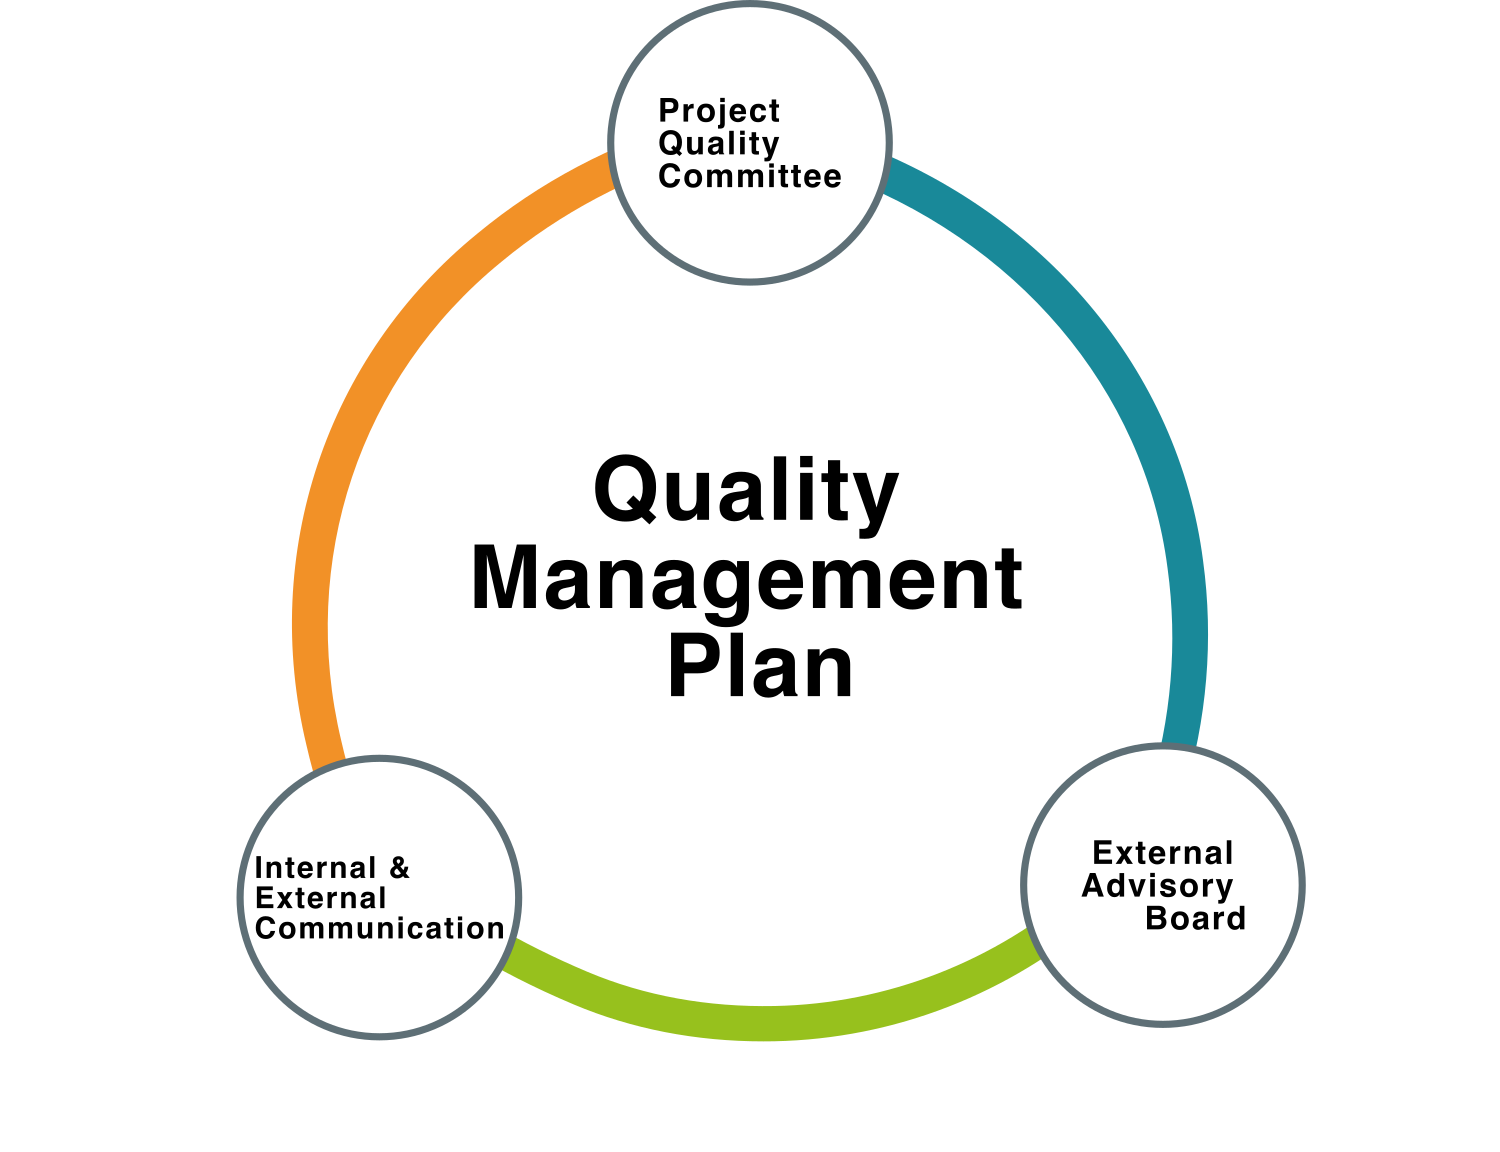
\includegraphics[width=0.6\linewidth,height=\textheight,keepaspectratio]{figures/6.1/Quality-management-plan.png}

}

\caption{\label{fig-qmp}Overview of the quality management plan.}

\end{figure}%

The quality system framework of the project is built around three key
components:

\begin{enumerate}
\def\labelenumi{\arabic{enumi}.}
\item
  \textbf{Project Quality Committee}: it is responsible for defining
  clear, open, and transparent governing principles at the outset of the
  project. These principles will ensure traceability and inclusivity in
  decision-making, allowing all partners to actively contribute to
  strategic discussions. The Université de Lorraine (UL), in
  collaboration with selected partners, will co-create a Quality Plan
  that defines the criteria, indicators, and procedures to guide the
  project's development and ensure high standards of quality.
\item
  \textbf{Communication Tools and Procedures}: UL will establish a
  shared digital platform to ensure that all relevant documents and
  materials are accessible to all consortium members. In addition, a
  monthly virtual meeting (minimum two hours) will be held to review
  progress, share updates, and coordinate upcoming tasks, fostering
  consistent communication and alignment across the consortium.
\item
  \textbf{External Advisory Committee}: An external committee, composed
  of independent experts, will be appointed to review and provide
  feedback on the project's public deliverables. Their role is to
  strengthen the project's external engagement and ensure its outputs
  meet high-quality standards and giving feedback on the TechTraPlastiCE
  development. A dedicated document outlining the tasks,
  responsibilities, and operational procedures of the advisory committee
  will be shared with all partners.
\end{enumerate}

The TechTraPastiCE project is strategically structured to maximize its
impact on the transition toward a Circular Economy in the Latin American
industrial plastic sector. Therefore, the quality efforts will ensure
the delivery of pertinent outcomes, support long-term capacity building,
and contribute to the development of sustainable interaction of the
academia with the socio-economic ecosystems. The following sections will
provide further detail on the implementation strategies, monitoring
mechanisms, and expected quality guidelines of the project.

\chapter{Project Quality Committee
--PQC-}\label{project-quality-committee-pqc-}

The Université de Lorraine is in charge of the coordination of the
project following the Grant Agreement and under the delegation of the
consortium members expressed through the mandates annexed to the Grant
Agreement. In that sense, UL will lead to establish a \textbf{Project
Quality Committee (PQC)} that will at the heart of the quality assurance
of the project outcomes.

This internal structure is entrusted with the revision and continuous
improvement of the project quality, which outlines specific standards,
processes, and responsibilities to be adhered to throughout the project
lifecycle. In the following subsections, an attention will be made to
the different guidelines for the PQC.

\section{Role and principles of the
PQC}\label{role-and-principles-of-the-pqc}

The major goals of the project quality committee regarding the
differents deliverables of TechTraPlastiCE project are:

\begin{enumerate}
\def\labelenumi{\arabic{enumi}.}
\item
  Deliverables are designed to enhance proficiency in project
  management, thereby supporting more effective project execution and
  oversight.
\item
  Deliverables meet the specific requirements of project lead
  beneficiaries, partners representatives, the project coordinator, and
  ultimately, the European Union.
\item
  Deliverables are aligned with industry best practices in project
  management, ensuring quality and consistency across project outputs.
\item
  Deliverables are prepared for web delivery and dissemination
  respecting the visual identity requirements (cf.~Deliverable 5.2),
  with the exception of those classified as confidential.
\item
  Deliverables are clear, comprehensive, and user-friendly. They provide
  all necessary information required by Partners to effectively progress
  in relevant tasks, minimizing the need for additional clarification,
  integration requests, or supplementary data.
\end{enumerate}

The PQC is established for the duration of the project, taking into
account three main roles:

\begin{enumerate}
\def\labelenumi{\arabic{enumi}.}
\tightlist
\item
  Validation the timely fulfillment of the tasks and obligations
  acquired by the partners are completed efficiently and effectively.\\
\item
  The quality approval of the working packages' deliverables assuring
  that both inputs and outputs are meet based on predefined performance
  criteria.
\item
  Identification of proactive actions if particular tasks will need
  additional support.
\end{enumerate}

These three elements are the heart of the quality management of the
project. Any proposed modifications to the quality plan must be formally
reviewed and approved through a defined revision process, led by the PQC
and finalized with the approval of the project coordinator.

This process ensures that all changes are tracked, documented, and
communicated clearly across the project team, reinforcing consistency
and traceability.

For doing that, five major principles will be assured throughout the
project duration in order to guarantee a pertinent quality management
process:

\begin{tcolorbox}[enhanced jigsaw, colframe=quarto-callout-note-color-frame, coltitle=black, rightrule=.15mm, bottomtitle=1mm, leftrule=.75mm, titlerule=0mm, opacitybacktitle=0.6, arc=.35mm, toprule=.15mm, bottomrule=.15mm, left=2mm, title=\textcolor{quarto-callout-note-color}{\faInfo}\hspace{0.5em}{Principles of TechTraPlastiCE Quality Committee}, colback=white, colbacktitle=quarto-callout-note-color!10!white, breakable, toptitle=1mm, opacityback=0]

\begin{itemize}
\item
  \textbf{Respect}: Understood as the consideration and appreciation of
  the work of the other actors involved in the project, as well as
  respect for the environment and activities that promote its
  appreciation and conservation.
\item
  \textbf{Transparency}: it specifies that any information addressed to
  the PQC, consortium, general public, or stakeholders of the project
  will be easily accessible and easy to understand, and clear language
  shall be used. This principle also stipulates free access to meeting
  minutes and always having a clear and honest response regarding
  decision-making mechanisms.
\item
  \textbf{Accountability}: it assigns clear roles, responsibilities, and
  performance expectations to each project partner and governing body.
  In the TechTraPlastiCE project, each institution is held responsible
  for their commitments, outputs, and use of resources. Mechanisms for
  regular performance evaluation, issue resolution, and corrective
  action are integral to this principle, ensuring that all project
  activities are conducted with integrity and aligned with agreed
  standards and objectives.
\item
  \textbf{Strategic Alignment}: it ensures that all project activities,
  decisions, and resource allocations are consistently guided by the
  project's overarching goals, priorities, and intended impacts. This
  principle implies that efforts remain focused, coherent, and capable
  of delivering measurable value throughout the project duration.
\item
  \textbf{Cooperation}: it emphasizes the importance of open dialogue,
  trust, and shared commitment among all partners of TechTraPlastiCE. It
  will foster a working environment where partners actively contribute
  to common goals, align efforts, and resolve challenges collectively
  ensuring that the project implementation will benefit from the
  collective expertise, resources, and engagement of the entire
  consortium.
\end{itemize}

\end{tcolorbox}

\section{Obligations of the PQC}\label{obligations-of-the-pqc}

The \textbf{Quality Committee} is entrusted with the following
responsibilities to ensure the effective implementation and high
standards of the project:

\begin{enumerate}
\def\labelenumi{\arabic{enumi}.}
\tightlist
\item
  Assess and validate the quality and timely completion of all
  deliverables within each work package, ensuring full compliance with
  the agreed project plan. When necessary, the Committee may seek the
  expertise of another project partner or a member of the
  \textbf{External Advisory Board} if the review requires additional
  technical or disciplinary competencies.
\end{enumerate}

\begin{enumerate}
\def\labelenumi{\arabic{enumi}.}
\tightlist
\item
  Oversee adherence to deadlines and monitor the progress of activities
  in accordance with the established project schedule, ensuring timely
  delivery of all expected outcomes.
\end{enumerate}

\begin{enumerate}
\def\labelenumi{\arabic{enumi}.}
\tightlist
\item
  Identify all scientific publications, books, and other outputs
  resulting from project activities. This assessment will be based on
  compliance with the Grant Agreement (notably Article I.16), alignment
  with the project's values and objectives, adherence to quality
  standards, and proper acknowledgment of all contributors.
\end{enumerate}

\begin{enumerate}
\def\labelenumi{\arabic{enumi}.}
\tightlist
\item
  Identify and propose appropriate measures to mitigate risks or respond
  to \textbf{force majeure}\footnote{See ARTICLE 35 --- FORCE MAJEURE of
    the EU Grants: AGA --- Annotated Grant Agreement: V2.0-- 01.04.2025.}
  events that could jeopardize the quality of deliverables or disrupt
  the project timeline. Eventually, conduct internal audits if repeated
  cases of non-compliance by consortium members are identified, in order
  to safeguard the integrity and accountability of the project.
\end{enumerate}

\section{Members of the PCQ}\label{members-of-the-pcq}

The project quality committee will be composed of 4 members of the
consortium of TechTraPlastiCE, two European and two from Latin-american
HEI as illustrated in Figure~\ref{fig-members}.

\begin{figure}[H]

\centering{

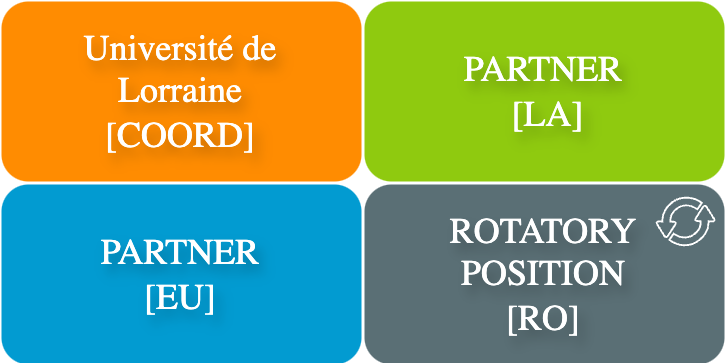
\includegraphics[width=0.6\linewidth,height=\textheight,keepaspectratio]{figures/6.1/PQC-00.png}

}

\caption{\label{fig-members}Members of the project quality committe of
TechTraPlastiCE.}

\end{figure}%

\begin{enumerate}
\def\labelenumi{\arabic{enumi}.}
\tightlist
\item
  The Université de Lorraine will have a permanent position on the
  quality committee as coordinator of the TechTraPlastiCE project
  \emph{{[}COORD{]}}.
\item
  One position representing an European partners \emph{{[}EU{]}}.
\item
  One position representing Latin American partners \emph{{[}LA{]}}.
\item
  A rotating position \emph{{[}RO{]}} will be assigned according to the
  status of the project. Based on the timetable of the project, the
  partners that has the most significant relevance in the implementation
  phase will be invited to the committee to inform the factual
  development of the tasks. This includes advances and difficulties
  found to take action proactively.
\end{enumerate}

Regarding the consolidation of the members of the PQC, an open call will
made at the begginning of the project to establish the first committee.
Then, there will be an open call at \emph{Month 18} to change the
participants.

On the other hand, regarding the {[}RO{]} position, it is suggested the
following rotation as illustrated in the Table~\ref{tbl-rotation}. In
the case that one of the participants of {[}EU{]} or {[}LA{]} takes the
position as {[}RO{]}, there will be an open call to the consortium in
order to restablish the composition of the quality committee. It is
established that the committee will internally validate the member to be
invited to the next cycle of the rotating position and agree on the
interest of the declared institution in participating.

\begin{table}

\caption{\label{tbl-rotation}Planification of rotation position in the
quality comittee}

\centering{

\centering\begingroup\fontsize{11}{13}\selectfont

\begin{tabular}[t]{>{\raggedright\arraybackslash}p{5cm}>{\raggedright\arraybackslash}p{3cm}}
\toprule
\begingroup\fontsize{12}{14}\selectfont \cellcolor{Naranja}{\textcolor{white}{\textbf{Partner}}}\endgroup & \begingroup\fontsize{12}{14}\selectfont \cellcolor{Naranja}{\textcolor{white}{\textbf{Time}}}\endgroup\\
\midrule
Universidad Nacional del Sur & M9 - M15\\
\midrule\addlinespace
Columbus & M15 - M21\\
\midrule\addlinespace
Universidad de Santiago de Chile & M24 - M30\\
\midrule\addlinespace
Universidad Nacional de Rio Negro & M30 - M36\\
\bottomrule
\end{tabular}
\endgroup{}

}

\end{table}%

\section{Initial set-up of the PQC}\label{initial-set-up-of-the-pqc}

An open call to all members of the consortium was made at the virtual
meeting of Monday 28/04 2025, Thus, the initial set-up quality committee
was made as follows:

\begin{enumerate}
\def\labelenumi{\arabic{enumi}.}
\tightlist
\item
  {[}COORD{]} : Université de Lorraine --UL-:

  \begin{itemize}
  \tightlist
  \item
    Main: \emph{Fabio A. Cruz Sanchez}
  \item
    Substitute: Université de Lorraine: \emph{Catalina Suescun}.
  \end{itemize}
\item
  {[}EU{]} : Columbus Association --COL-

  \begin{itemize}
  \tightlist
  \item
    Main: \emph{Kelly Henao}
  \item
    Substitute: \emph{Cecilia Valdés}
  \end{itemize}
\item
  {[}LA{]} : Universidad Nacional de Rio Negro --UNRN-

  \begin{itemize}
  \tightlist
  \item
    Main: \emph{Marian Lenchours Pezzano}
  \item
    Substitute: \emph{Maria Paula Awe Luca}
  \end{itemize}
\item
  {[}RO{]} : Pontificia Universidad de Valparaiso --PUCV-:

  \begin{itemize}
  \tightlist
  \item
    Main: \emph{Sandra Ponce}
  \item
    Substitute: \emph{Carlos Calesi}
  \end{itemize}
\end{enumerate}

Regarding the {[}RO{]} position, the Pontificia Universidad de
Valparaiso - Chile was proposed initially as they will lead the WP1 in
the first phase of the project.

\section{Procedures of the PQC}\label{procedures-of-the-pqc}

\begin{figure}[H]

\centering{

\pandocbounded{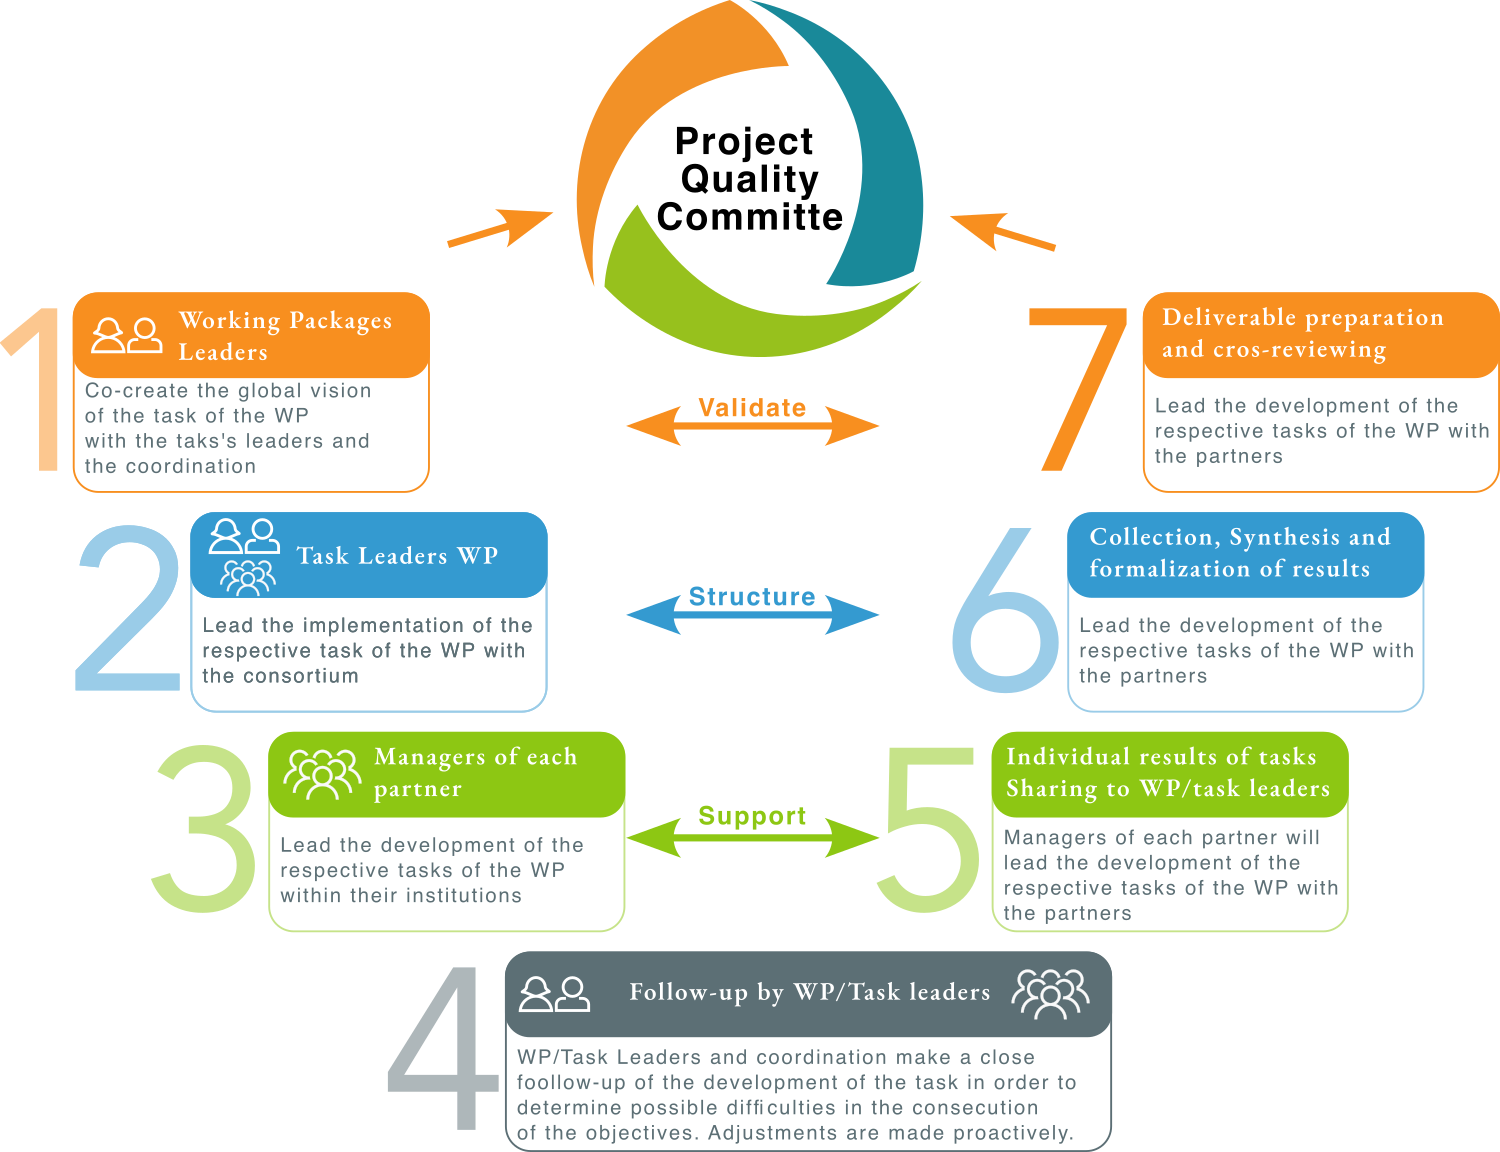
\includegraphics[keepaspectratio]{figures/6.1/Procedure-PQC.png}}

}

\caption{\label{fig-pqc-procedure}Procedure of the quality management of
the TechTraPlastiCE development}

\end{figure}%

Figure~\ref{fig-pqc-procedure} illustrates the procedure of the
delevopment of the TechTraPlastiCE project. Each step present the
objective expected.

\begin{enumerate}
\def\labelenumi{\arabic{enumi}.}
\tightlist
\item
  \emph{Step 1}: aims that WP leaders interact with the task leaders and
  the coordination before the WP starts in order to define the shared
  language and vision for the WP.
\item
  \emph{Step 2}: seeks to task leader organize and structure the
  instruments to be used with th thewhole consortium to the development
  of the tasks.
\item
  \emph{Step 3}: Managers of each partners will lead the implementation
  of the task within its local university/ecosystem taking the support
  of the leaders tasks.
\item
  \emph{Step 4}: The participants develop the respective tasks according
  to the indications of task leaders.
\item
  \emph{Step 5}: Manager of each university will collect, synthethise
  and share the results with the task leaders.
\item
  \emph{Step 6}: Task leaders will formalize the set of results obtained
  by the consortium, validating the respective objectives and
  milestones.
\item
  \emph{Step 7}: WP and task leaders will formalize the deliverable to
  be share to the PCP and for the cross-reviewing process before
  submission to the EU commission.
\end{enumerate}

Based on that process, the quality committee will promote a quick and
effective identification of the problems during the project. It aims to
co-create solutions between the parties in case of disagreements and
divergence of perspectives in the project development. If consortium
partners present different criteria, therefore conflict resolution
policies shall be applied following the protocol as follows:

\begin{enumerate}
\def\labelenumi{\arabic{enumi}.}
\tightlist
\item
  In case of conflict, dialogue takes place with the work package leader
  and the partner' managers. If necessary, the project coordinator can
  participate.
\item
  If the conflict resolution is not in the hands of the project
  coordinator, the case will be presented to the quality committee. The
  quality committee will make decisions based on a simple majority (3 of
  4 members), and each member has one vote.
\item
  The quality committee can decide to open the space for resolution,
  calling an extraordinary assembly of all members and requesting
  arbitration or advice from the External Advisory Board.
\end{enumerate}

Any difference resulting from this plan's interpretation or application
will be resolved by direct negotiation between the parties. At any time,
a consortium partner may propose, by formal communication, to the
quality committee its modification.

The quality committee will decide in the closest ordinary session
whether or not to approve the requested modification. Any modification
must be framed within the objectives and results established in the
project, Grant Agreement, and general guidelines of the Capacity
Building in the field of higher education 2025 of the Education,
Audiovisual and Culture Executive Agency --EACEA-.

\section{Official Meetings of the
PQC}\label{official-meetings-of-the-pqc}

As a general rule, at least one official meeting per semester will be
made in order to guarantee the advancement of the project.
Table~\ref{tbl-meetings} present an proposition of expected meetings
will take place during the project. This is a first draft proposition
that will evolve during the project development. The call for sessions
of the quality committee will be notify by the Coordinator at least
\emph{fifteen days} in advance.

\begin{table}

\caption{\label{tbl-meetings}Planification of Official Meetings of the
project quality committee}

\centering{

\centering\begingroup\fontsize{11}{13}\selectfont

\begin{tabular}[t]{>{\centering\arraybackslash}p{1.5cm}>{\centering\arraybackslash}p{2cm}>{\raggedright\arraybackslash}p{7cm}}
\toprule
\begingroup\fontsize{12}{14}\selectfont \cellcolor{Naranja}{\textcolor{white}{\textbf{Meeting}}}\endgroup & \begingroup\fontsize{12}{14}\selectfont \cellcolor{Naranja}{\textcolor{white}{\textbf{Expected date}}}\endgroup & \begingroup\fontsize{12}{14}\selectfont \cellcolor{Naranja}{\textcolor{white}{\textbf{Possible Agenda}}}\endgroup\\
\midrule
1 & M6 & 1) Task of WP1 and links WP1 and WP2 \newline  2) Establishment of supporting task fo WP5 and WP6\\
\midrule\addlinespace
2 & M12 & 1) Tasks of WP2 \newline  2) Connection of inputs of WP1 / WP2 for WP3\\
\midrule\addlinespace
3 & M18 & 1) Development of  WP3.\newline  2) Intermediate Rapport\\
\midrule\addlinespace
4 & M27 & 1) Implementation of WP4.\newline  2) Data collection from WP4 for final rapport\\
\midrule\addlinespace
5 & M33 & 1) Final conferences.\newline  2) Public results and outputs\\
\bottomrule
\end{tabular}
\endgroup{}

}

\end{table}%

The committee may meet in extraordinary sessions called when one of the
members of the committee so requires, after notification via email,
justifying the need for the session and at least ten days in advance.

The committee will meet with a quorum of \emph{at least three members},
and in the absence of a quorum, the committee shall be summoned again
within the next 10 days. The leaders of the work packages will be
summoned to accompany the quality committee sessions when necessary. The
leaders of the aforementioned work packages will participate with voice,
but will not have a vote in the decisions that are determined in the
committee.

\section{Quality Guidelines}\label{quality-guidelines}

The quality guidelines of the TechTraPlastiCE project are not limited to
the end results or deliverables; but rather, the purpose is to have an
integral consideration across every phase of the project, from planning,
execution and evaluation of each tasks.

In that sense, based on the timetable plan and on the Logical Framework
Matrix the proposal, the quality committe will help to assess
expectations, level of progress and difficulties of each task and
milestone .\\
Additionally, in the regular consortium planned meetings (virtual and
physical), the checking progress and difficulties of the work packages
will be monitored. Therefore, two major approaches are envisaged:

\begin{enumerate}
\def\labelenumi{\arabic{enumi}.}
\tightlist
\item
  The quality processes of the project are based on internal monitoring.
\item
  Cross-revision of the deliverables by the consortium before
  sumbmission.
\end{enumerate}

\subsection{Internal monitoring}\label{internal-monitoring}

In the physical meetings planned by in the TechTraPlastiCE, the progress
and difficulties of the work packages will be internally monitoring by
the project quality committee. Thus, Table~\ref{tbl-int.monitoring}
presents the guideline points to be discussed in each event. Appropriate
instruments will be structured for those sessions with the whole
consortium to especify the quality of the tasks.

\begin{table}[H]

\caption{\label{tbl-int.monitoring}Guideline points of the PCQ at the
event meetings}

\centering{

\centering\begingroup\fontsize{11}{13}\selectfont

\begin{tabular}[t]{>{\raggedright\arraybackslash}p{3cm}>{\raggedright\arraybackslash}p{2cm}>{\raggedright\arraybackslash}p{8cm}}
\toprule
\begingroup\fontsize{12}{14}\selectfont \cellcolor{Naranja}{\textcolor{white}{\textbf{Meeting}}}\endgroup & \begingroup\fontsize{12}{14}\selectfont \cellcolor{Naranja}{\textcolor{white}{\textbf{Place}}}\endgroup & \begingroup\fontsize{12}{14}\selectfont \cellcolor{Naranja}{\textcolor{white}{\textbf{Quality points}}}\endgroup\\
\midrule
Kick-off Meeting & Nancy - France & 1) Baseline and expectations on the project as a whole.\newline  2) Connection with local ecosystems of plastic value\\
\midrule\addlinespace
Pre-definition of portfolios & Santiago de Chile, Chile & 1) Integration of University to the project\\
\midrule\addlinespace
Pilots implementation follow-ups & Bogota, Colombia & 1) Definition and adequation of  the pilots projects \newline  2) Follow up of the development\\
\midrule\addlinespace
Pilot results and dissemination & Bariloche, Argentina & 1) Validation of the results and learned lessons among the three countries.\\
\bottomrule
\end{tabular}
\endgroup{}

}

\end{table}%

On the other hand, the following factual elements will be used as
primary sources of analysis:

\begin{enumerate}
\def\labelenumi{\arabic{enumi}.}
\tightlist
\item
  \textbf{\emph{Report of the work packages leaders:}} the leaders of
  the work packages must give a feedback to the quality committee on the
  progress and execution of their activities. In each monthly meeting is
  expected to give time for the development of each task that is running
  according to the timetable of the project.
\item
  \textbf{\emph{Tools and Instruments}}: Response rate of the project
  instruments (i.e.~online questionnaires / surveys, physical meetings
  among others) developed by the consortium.
\item
  \textbf{\emph{Interviews}}: specific meetings with the task and work
  packages leaders in each institution.
\item
  \textbf{\emph{Focus groups}}: during the development of the
  TechTraPlastiCE project, it is intended integrate external
  stakeholders in particular task (i.e: search conferences, Creativity
  solving challenges analysis in different meetings of the project.)
\item
  Other tools agreed upon by the Quality Committee.
\end{enumerate}

As secondary information, the following will be used:

\begin{itemize}
\tightlist
\item
  Progress reports and institutional documents of the partners used for
  internal monitoring and quality assurance.
\item
  Analysis of the minutes of the development of the tasks.
\end{itemize}

Based on these elements, the internal monitoring of the project will
take place for the official meetings of the quality committee.

\subsection{Working Packages Leaders and Cross-reviewing process of
deliverables}\label{working-packages-leaders-and-cross-reviewing-process-of-deliverables}

TechTraPlastiCE project will implement an internal cross-reviewing of
each deliverable before they are submitted to the official EU portal.
Therefore, each partner will have a role as a reviewer. In that sense,
the expected role of the cross-reviewer is to seek coherence in the
content, structure, and formatting of the deliverable, ensuring
alignment with the project objectives, work package descriptions, and EU
guidelines. Reviewers will verify the accuracy of technical information,
clarity of language, and consistency across sections. Feedback will be
provided in a timely manner using a standardized review template to
ensure a harmonized approach across all partners using the format in the
Section~\ref{sec-cross}.

Thus, it is the responsibility of the Work Package Leader to coordinate
the delivery dates, results, and established activities, and ensuring
the quality of the deliverables in charge of others involved in the work
package activities. Consequently, it is the responsibility of the
deliverables leader to planify, prepare and develop the respective
document for WP leader.

The WP leaders must send the final version of the documents of their
package to the Quality Committee and the specific partner designed for
the internal reviewing according to Table~\ref{tbl-int.cross}. In the
event of any delay, it is possible to write to the project coordinator
explaining the reasons. The coordination can grant an extra delay of 5
days without the need to consult with the Quality Committee. A more
extended period must be consulted with the Quality Committee.

The coordinatiion will oversee the review process and ensure the
incorporation of relevant feedback before final submission. This quality
management process aims to enhance the reliability, professionalism, and
impact of all project outputs while fostering mutual accountability and
collaboration among partners throughout the project's duration.

In the event of force majeure that makes it impossible to comply with
the activities and deliverables established in the work package, the
package leader must notify the project coordinator who will replicate
the information to the quality committee to validate strategies that
ensure the successful completion of the project.

\begingroup\fontsize{11}{13}\selectfont

\begin{longtable}[t]{>{\centering\arraybackslash}p{0.8cm}>{\centering\arraybackslash}p{2cm}>{\raggedright\arraybackslash}p{6cm}>{\raggedright\arraybackslash}p{3cm}>{\raggedright\arraybackslash}p{3cm}|}

\caption{\label{tbl-int.cross}Internal cross-reviewing process for the
deliverables of TechTraPlastiCE}

\tabularnewline

\toprule
\begingroup\fontsize{12}{14}\selectfont \cellcolor{Naranja}{\textcolor{white}{\textbf{No}}}\endgroup & \begingroup\fontsize{12}{14}\selectfont \cellcolor{Naranja}{\textcolor{white}{\textbf{Deliverable}}}\endgroup & \begingroup\fontsize{12}{14}\selectfont \cellcolor{Naranja}{\textcolor{white}{\textbf{Deliverable Name}}}\endgroup & \begingroup\fontsize{12}{14}\selectfont \cellcolor{Naranja}{\textcolor{white}{\textbf{Lead Beneficiary}}}\endgroup & \begingroup\fontsize{12}{14}\selectfont \cellcolor{Naranja}{\textcolor{white}{\textbf{Cross-reviewing}}}\endgroup\\
\midrule
\endfirsthead
\multicolumn{5}{@{}l}{\textit{(continued)}}\\
\toprule
\begingroup\fontsize{12}{14}\selectfont \cellcolor{Naranja}{\textcolor{white}{\textbf{No}}}\endgroup & \begingroup\fontsize{12}{14}\selectfont \cellcolor{Naranja}{\textcolor{white}{\textbf{Deliverable}}}\endgroup & \begingroup\fontsize{12}{14}\selectfont \cellcolor{Naranja}{\textcolor{white}{\textbf{Deliverable Name}}}\endgroup & \begingroup\fontsize{12}{14}\selectfont \cellcolor{Naranja}{\textcolor{white}{\textbf{Lead Beneficiary}}}\endgroup & \begingroup\fontsize{12}{14}\selectfont \cellcolor{Naranja}{\textcolor{white}{\textbf{Cross-reviewing}}}\endgroup\\
\midrule
\endhead

\endfoot
\bottomrule
\endlastfoot
D1 & D1.1 & Framework to understand barriers and benefits to apply with local legislation & PUCV & \cellcolor{Verde}{\textbf{UNAL}}\\
\midrule\addlinespace
D2 & D1.2 & A document containing the gap analysis for companies/industries & PUCV & \cellcolor{Verde}{\textbf{UNS}}\\
\midrule\addlinespace
D3 & D1.3 & Results of the application of the innovation metrology index to target industries of the plastic value chain & UL & \cellcolor{Verde}{\textbf{UC}}\\
\midrule\addlinespace
D4 & D2.1 & Repository with proposed solutions/services & UA & \cellcolor{Verde}{\textbf{UNRN / UL}}\\
\midrule\addlinespace
D5 & D2.2 & Document with Portfolio definition by Institution & UNS & \cellcolor{Verde}{\textbf{UNRN / PUCV}}\\
\midrule\addlinespace
D6 & D2.3 & Mentoring  and peer-collaboration learning reports & UNS & \cellcolor{Verde}{\textbf{UNC}}\\
\midrule\addlinespace
D7 & D3.1 & Comprensive problem definition on the reuse challenge & COLUMBUS & \cellcolor{Verde}{\textbf{UNAL / USACH / UNS}}\\
\midrule\addlinespace
D8 & D3.2 & Report on contacts and results of interviews & PUCV & \cellcolor{Verde}{\textbf{UL}}\\
\midrule\addlinespace
D9 & D3.3 & Benchmarking study & PUCV - COLUMBUS & \cellcolor{Verde}{\textbf{UA}}\\
\midrule\addlinespace
D10 & D3.4 & 4 Events reports (One per institution) & COLUMBUS & \cellcolor{Verde}{\textbf{UC / UNRN / PUCV}}\\
\midrule\addlinespace
D11 & D3.5 & Updated portfolios & UNS & \cellcolor{Verde}{\textbf{UA / UNC}}\\
\midrule\addlinespace
D12 & D4.1 & Report of the creative-based challenges to integrate Industry-University & USACH & \cellcolor{Verde}{\textbf{UC}}\\
\midrule\addlinespace
D13 & D4.2 & Pilots definition documents & UNS & \cellcolor{Verde}{\textbf{COLUMBUS}}\\
\midrule\addlinespace
D14 & D4.3 & Digital Notebook with lessons and support actions & UC & \cellcolor{Verde}{\textbf{UNC}}\\
\midrule\addlinespace
D15 & D4.4 & Document with recommendations & COLUMBUS & \cellcolor{Verde}{\textbf{UNAL / UNS / PUCV}}\\
\midrule\addlinespace
D16 & D5.1 & Document with the dissemination digital strategy & UNRN & \cellcolor{Verde}{\textbf{USACH}}\\
\midrule\addlinespace
D17 & D5.2 & Branding digital material and training program & UNRN & \cellcolor{Verde}{\textbf{USACH}}\\
\midrule\addlinespace
D18 & D5.3 & Project Website and Social Media accounts & UNRN & \cellcolor{Verde}{\textbf{UL}}\\
\midrule\addlinespace
D19 & D5.4 & Repository with materials & UL & \cellcolor{Verde}{\textbf{UNC}}\\
\midrule\addlinespace
D20 & D5.5 & Final conference document results & UNRN & \cellcolor{Verde}{\textbf{UA / UNAL}}\\
\midrule\addlinespace
D21 & D6.1 & Quality assurance plan & UL & \cellcolor{Verde}{\textbf{COLUMBUS}}\\
\midrule\addlinespace
D22 & D6.2 & Financial and technical management & UL & \cellcolor{Verde}{\textbf{COLUMBUS}}\\
\midrule\addlinespace
D23 & D6.3 & Midterm Progress report & UL & \cellcolor{Verde}{\textbf{ALL}}\\*

\end{longtable}

\endgroup{}

Finally, the WP leaders will share to all partners around progress,
results, risks, and risk mitigation proposals of the delvepment of each
deliverable.

\chapter{Internal and External Communications \&
Publications}\label{internal-and-external-communications-publications}

Regarding the means of communication, the coordination will guarantee
the technological infrastructure to make possible the meetings of the
quality committee. Each meeting will be documented with an
action-oriented \emph{compte rendu}, not only to a report with general
information on project activities but also includes risk analysis and
timely. The internal quality findings will be formally documented and
communicated across the project governance structure providing a quick
overview and facilitates communication with partners, and facilitates
the decision-making process.

\section{Internal communication}\label{internal-communication}

Table~\ref{tbl-int.comm} presents the various methods of communication
among the TechTraPlastiCE consortium. These communication methods
provide standards for information exchange, ensuring that the
participants in the task, and affected groups are informed on the
appropriate aspects of project and intergroup commitments are
communicated.

\begingroup\fontsize{11}{13}\selectfont

\begin{longtable}[t]{>{\raggedright\arraybackslash}p{2cm}>{\raggedright\arraybackslash}p{3cm}>{\raggedright\arraybackslash}p{6cm}>{\raggedright\arraybackslash}p{3cm}}

\caption{\label{tbl-int.comm}Communication Methods of TechTraPlastiCE}

\tabularnewline

\toprule
\begingroup\fontsize{12}{14}\selectfont \cellcolor{Naranja}{\textcolor{white}{\textbf{From}}}\endgroup & \begingroup\fontsize{12}{14}\selectfont \cellcolor{Naranja}{\textcolor{white}{\textbf{To}}}\endgroup & \begingroup\fontsize{12}{14}\selectfont \cellcolor{Naranja}{\textcolor{white}{\textbf{Function}}}\endgroup & \begingroup\fontsize{12}{14}\selectfont \cellcolor{Naranja}{\textcolor{white}{\textbf{Frequency}}}\endgroup\\
\midrule
\endfirsthead
\multicolumn{4}{@{}l}{\textit{(continued)}}\\
\toprule
\begingroup\fontsize{12}{14}\selectfont \cellcolor{Naranja}{\textcolor{white}{\textbf{From}}}\endgroup & \begingroup\fontsize{12}{14}\selectfont \cellcolor{Naranja}{\textcolor{white}{\textbf{To}}}\endgroup & \begingroup\fontsize{12}{14}\selectfont \cellcolor{Naranja}{\textcolor{white}{\textbf{Function}}}\endgroup & \begingroup\fontsize{12}{14}\selectfont \cellcolor{Naranja}{\textcolor{white}{\textbf{Frequency}}}\endgroup\\
\midrule
\endhead

\endfoot
\bottomrule
\endlastfoot
Project Coordination & All consortium & Intergroup coordination, \newline  Status of critical tasks & Monthly\\
\midrule\addlinespace
WP Leaders & All consortium & Reporting of task advancements \newline  Communication insigths & Bi-weekly\\
\midrule\addlinespace
WP Leaders & Project Coordination & Adequation of task projects \newline  Follow up of the development & Bi-weekly\\
\midrule\addlinespace
WP Leaders & Managers of each partner & Task development \newline  Follow up of results & Weekly\\*

\end{longtable}

\endgroup{}

Day by day communication of Project related issues will be done via
email/ phone. Important communications should be traced via mail with
copy to Coordinator.

\section{External Communication}\label{external-communication}

On the other hand, regarding the external communications, all partner of
the consortium must pay special attention to the general guidelines of
the financing instrument ``Capacity Building in the field of higher
education 2025'' of the EACEA of the European Community and the
provisions of the Grant Agreement, in particular, what is mentioned in
Article 17 on \emph{Communication, Dissemination and Visibility}.

All members of the project, coordinating institutions, partners,
consultants, and external stakeholders must be aware of these guidelines
modifications and be co-responsible for the general quality of the
deliverables, dissemination, internal and external meetings.

Each Partner wishing to undertake any formal communication
activity/initiative related to the Project should inform WP5 Lead
Beneficiary (Universidad Nacional de Rio Negro --UNRN-) as leader of
dissemination activities.

The content and the overall message of the communication activities
should be agreed with the WP5. Lead Beneficiary should be consulted on
the visual identity of the Project (logo, communication style..). All
communication activities shall be monitored by the UNRN at latest
quarterly.

\section{Dissemination and publication of project
results}\label{dissemination-and-publication-of-project-results}

Before the dissemination and publication of project results, the partner
shall give the Coordinator and all the other Project Partners at least
30-calendar-day-notice.

Other Partners then have two calendar weeks to comment the
dissemination/publication and request necessary modifications, if any.
If there are no Partners comments within the period above, the
dissemination/publication of results is allowed.

\section{Use of social media}\label{use-of-social-media}

The Project uses social media. Any content to be shared using social
media shall be sent in advance to the WP5 Leader (UNRN).

\chapter{External Advisory Board}\label{external-advisory-board}

The quality control and monitoring processes will identify both
qualitative and quantitative data collected from all project partners
and key stakeholders based on specific criteria:

\begin{enumerate}
\def\labelenumi{\arabic{enumi}.}
\tightlist
\item
  Relevance: Evaluate the alignment of objectives with the needs and
  priorities of the partners.
\item
  Effectiveness: Examine whether the project outputs are contributing to
  the achievement of projected outcomes and meeting its objectives.
\item
  Pertinence: Assess the relevance, usefulness, and efficiency of inputs
  in delivering outputs in an economical and timely manner.
\item
  Collaboration and Communication: Assessing the effectiveness of
  communication channels and collaboration among project partners,
  ensuring transparent information exchange, and fostering a cohesive
  working environment conducive to achieving project objectives.
\item
  Continuous Improvement: Implementing mechanisms for ongoing evaluation
  and feedback loops to identify areas for improvement and optimize
  project processes, fostering a culture of continuous learning and
  enhancement throughout the project lifecycle.
\end{enumerate}

In that sense, a dedicated \textbf{External Advisory Board (EAB)} will
be established, composed of five high-level experts from relevant
fields. The main objective of the EAB is to provide independent,
strategic advice to the project consortium based on the obtained data,
thereby enhancing the overall scientific and societal impact of the
initiative.

The EAB will serve as a critical interface between the TechTraPlastiCE
consortium and external stakeholders, offering guidance on key issues,
responding to consortium queries, and contributing to the broader
dissemination and visibility of project results. Its role will be
instrumental in aligning project activities with current trends, best
practices, and emerging opportunities in the field, especially at the
European and global levels.

Members of the EAB will be selected for their expertise and professional
standing in areas directly relevant to the core objectives of the
project. Particular focus will be placed on:

\begin{enumerate}
\def\labelenumi{\arabic{enumi}.}
\item
  \textbf{Technological transfer and academia-industry collaboration} :
  experts in these competences will TechTraPlastiCE consortium to
  adquire effective knowledge onthe different transfer mechanisms and
  partnerships and their limitations. This is important in the sscope of
  the project.
\item
  \textbf{Circular economy within the plastic value chain}: experts in
  cricular economy could bring to the consortium examples of sustainable
  practices, lifecycle thinking, and resource efficiency where the
  academia can collaborate with the socio-economical actors.
\item
  \textbf{Integration of marginalized actors in the plastic value chain
  into academic and research ecosystems} : experts in this topic can
  illustrated the consortium, and more particular the latinamerican
  context, the relevant role of inclusivity, equity, and capacity
  building for underrepresented communities in the circular economy.
  This is a major competence where the shared of experiences will have a
  major impact inside and outside of the consortium.
\end{enumerate}

The EAB will work closely with the project coordinator and select
members of the consortium. \textbf{Two formal meetings per year} will be
coordinated by the project coordinator, although \textbf{ad hoc
consultations} may occur as needed. In addition to strategic input, EAB
members will also be invited to participate in key project events,
workshops, and public engagement activities, thereby contributing to
increased visibility and uptake of project outcomes across multiple
sectors.

By incorporating diverse perspectives and expertise, the
\textbf{External Advisory Board} will play a vital role in reinforcing
the relevance, inclusiveness, and long-term sustainability of
TechTraPlastiCE's results.

The settting up proposition

As example, during the kick of meeting, we had the opportunity to invite
Prof.~Ferran Giones\footnote{See her profile on
  \url{https://www.gu.se/en/about/find-staff/mariajosezapatacampus}} of
the university of Sttutgart and the Prof.~Maria Jose Zapata\footnote{See
  his profile on
  \url{https://www.eni.uni-stuttgart.de/en/institute/team/Giones/}} of
the University of Gottemburg. They share with the TechTraPlastiCE
consortium a presentation on ``\emph{Technology Transfer Challenges \&
Opportunities}''\,'' (Prof.~Feeran Giones) and ``\emph{Circular
Grassroots Innovations}'' (Prof.~Marioa Jose Zapata); giving remarkables
insigths in the challenges that TechTraPlastiCE aims to tackle.

\begin{figure}[H]

{\centering \pandocbounded{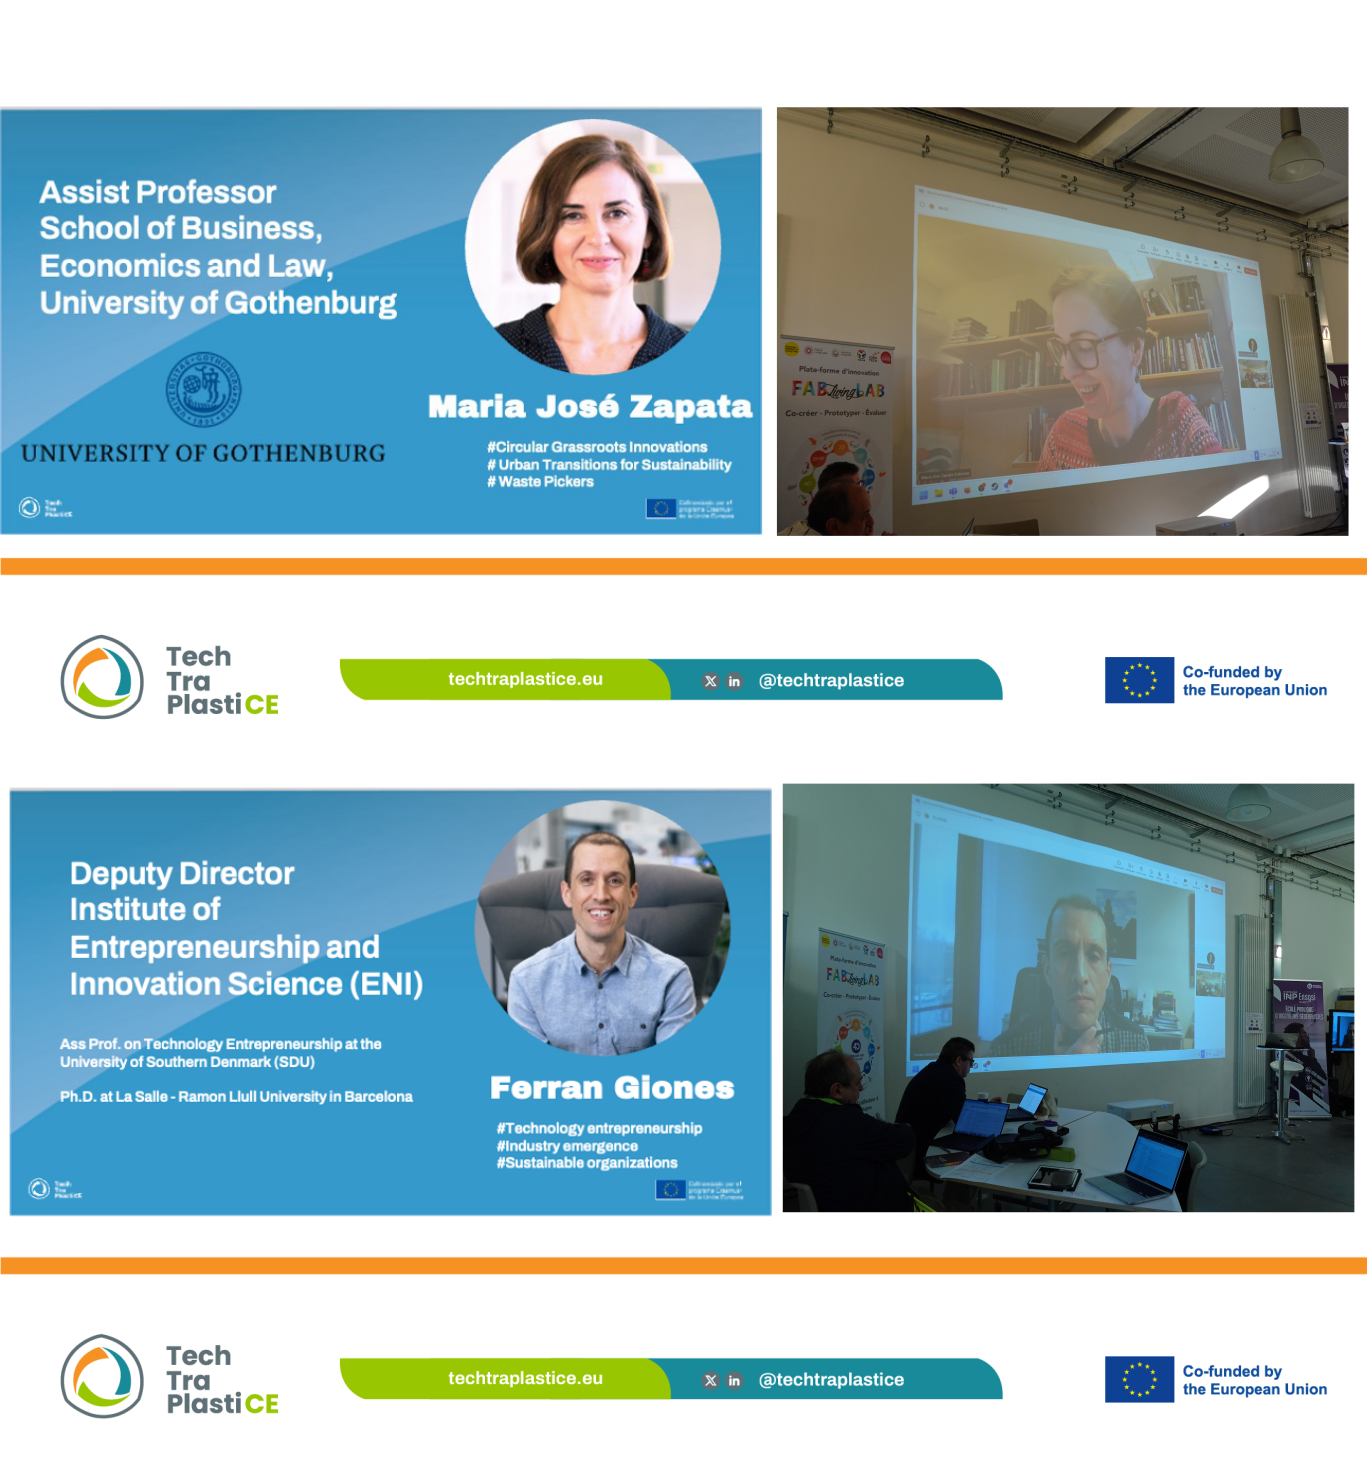
\includegraphics[keepaspectratio]{figures/6.1/External-committe.png}}

}

\caption{Participation of Prof.~Ferran Giones from University of
Sttutgart and Prof.~Maria José Zapata from the University of Gotemburg
during Kick-off meeting at Nancy, France on March 25-28/2025.}

\end{figure}%

\chapter{Conclusions}\label{conclusions}

This document reports a quality plan that will be implememented in the
TechTrasPlastiCE project. The quality plan will take three major
elements, namely 1) quality committee project that establish an overall
governance of the quality aspect of the project, 2) internal and
external communications and 3) external advisory committee.

These elements aims to provide sufficient mechanisms and instruments
approved by mutual agreement to ensure compliance with the project's
objectives and indicators with high-quality standards and delimiting
decision-making elements. Also, it will specify the means of
communication, frequency and the external advisory board that will join
the project to guarantee the outputs of the project implementation.

\appendix

\chapter{Annexes}\label{annexes}

\section{Review report in the cross-evaluation process}\label{sec-cross}

\begin{Form}
\begin{tabular}{p{15cm}}
\toprule
   \TextField[width=6cm]{Title of deliverable: } \\
   \TextField[width=3cm]{Date and Version of deliverable:} \\
   \TextField[width=6cm]{Deliverable description (from DoA)} \\
   \TextField[width=6cm]{Names of Reviewer} \\

\midrule
General questions to consideration: \\

Is the content of the deliverable exhaustive reagarding the DoA?\\
\TextField[width=\linewidth, height=2cm]{} \\
Is the deliverable easy to read (accessible wording, good structure), does it have a unified tone?\\
\TextField[width=\linewidth, height=2cm]{} \\
Is the content of the deliverable exhaustive? \\
\TextField[width=\linewidth, height=2cm]{} \\
Is the summary of the deliverable clear, concise and informative?\\
\TextField[width=\linewidth, height=2cm]{} \\
Please indicate strengths and weaknesses of the deliverable? \\
\TextField[width=\linewidth, height=2cm]{} \\

\bottomrule    
\end{tabular}
\end{Form}


\backmatter


\end{document}
